% set home directory
\providecommand{\homedir}{..} 
% load the preamble of main.tex by subfiles
\documentclass[\homedir/main.tex]{subfiles}
% ##############################################################################
\begin{document}
% set chapter numbering to work correctly even when separate compilation using subfile
\setcounter{chapter}{0}
% ##############################################################################
\chapter{序論}\label{chap:introduction}

\section{研究背景}\label{sec:background}
現代では,我々はしばしば色やエフェクトなどによって飾り付けられた文字を目にする.
このように装飾された文字は「デザイン文字」と呼ばれる.
デザイン文字は装飾のないシンプルな文字と比べ,目立ちやすく具体的なイメージを与えやすい点で優れている.
例えば,次の\cref{fig:design_char_eg}は赤い「炎」という文字に燃えているようなエフェクトを付与したものであるが,
装飾のない「炎」に比べメラメラと炎が燃えている印象が相手に良く伝わると考えられる.

\begin{figure}[h]
    \centering
    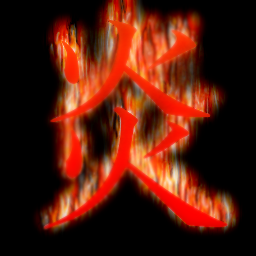
\includegraphics[keepaspectratio, scale=1.0]{design_character_example.png}
    \caption{デザイン文字の例}
    \label{fig:design_char_eg}
\end{figure}

そのため,デザイン文字は特に目立たせたい文字や印象づけたい文字に用いられている.
特に,作品のタイトル・企業名・商品名などのロゴは,印象に残ることが重要なためデザイン文字が用いられることが多い.
一方,そうしたデザイン文字の作成には高度な技術や多大な時間を要することも多い.
したがって,デザイン文字の作成手法の研究には意義がある.

ここで,実際にデザイン文字が用いられる場面を想定すると,
単一の文字としてではなく,複数文字からなる文字列として用いられることが多いと予想できる.
ゆえに,デザイン文字の作成手法よりも「デザイン文字列」の作成手法は有用だといえる.

但し,ここで言う「デザイン文字列」はデザイン文字を単に並べてできる文字列とは少し異なる.
それは,デザイン文字列にしかない要素がいくつか存在するからである.
ここでは,デザイン文字列にしかない要素の例を三つ挙げる.

一つ目は,文字同士の間隔である.
文字同士の間隔は通常の文書でも与える印象を左右する要素であるが,
デザイン文字列においても同様に印象を左右する要素である.

二つ目は,文字の配置である.
デザイン文字列では,文字列を構成する文字の配置を複雑にすることがある.
次の\cref{fig:X}はその一例である.

\begin{figure}[h]
    \centering
    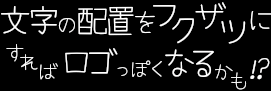
\includegraphics[keepaspectratio, scale=1.0]{place_char_example.png}
    \caption{文字の配置が複雑なデザイン文字の例}
    \label{fig:X}
\end{figure}

この\cref{fig:X}のようなデザインは昨今のアニメ作品のロゴに用いられている場合がある.

三つ目は,文字列の形状の歪みである.
デザイン文字列では,目を引くデザインとするために敢えて文字列を歪ませることがある.
次の\cref{fig:warp_txt_eg}はその一例である.

\begin{figure}[h]
    \centering
    
\includegraphics[keepaspectratio, width=0.7\linewidth]{warped_text_example.png}
    \caption{形状の歪みをもつデザイン文字列の例}
    \label{fig:warp_txt_eg}
\end{figure}

この\cref{fig:warp_txt_eg}のようなデザインはロゴの他にチラシなどで用いられることがある.

以上で述べたように,デザイン文字列には多種多様なものが存在する.
そして,より多種多様なデザイン文字列の自動作成を可能とするために手法を研究することには意義がある.

% ##############################################################################
\section{研究目的}\label{sec:objective}
\cref{chap:related_works}で詳述するが,
\cref{sec:background}で述べたようなデザイン文字列をStyle Transferを用いて作成する研究の先行研究は,
筆者の調査した限りでは見当たらなかった.
そのため,デザイン文字列を対象とすることには新規性が認められる.

そこで,本研究の目的は「デザイン文字列を別のデザイン文字や文字列画像をもとに
Style Transferを用いて自動で作成する手法の開発」とする.
なお,本研究ではデザイン文字列に特有の要素のうち,特に文字列全体の形状の歪みを扱うとする.

% ##############################################################################
\section{本論文の構成}\label{sec:structure}
本論文の構成は次のようになっている.
\cref{chap:introduction}では本研究の背景と目的を述べた.
\cref{chap:related_works}では本研究に関連する先行研究を紹介する.
\cref{chap:theories}では本研究の前提知識となる理論について述べる.
\cref{chap:methods}では本研究が提案する手法について述べる.
\cref{chap:experiment}では本研究で実施した評価実験の内容とその結果を述べる.
最後に,\cref{chap:summary}では本論文の結論と今後の課題を述べる.

% ##############################################################################
\printBibForSubfiles
\end{document}